\documentclass{beamer}
\usetheme[pageofpages=of,% String used between the current page and the
                         % total page count.
          bullet=circle,% Use circles instead of squares for bullets.
          titleline=true,% Show a line below the frame title.
          alternativetitlepage=true,% Use the fancy title page.
       %   titlepagelogo=logo-polito,% Logo for the first page.
       %   watermark=watermark-polito,% Watermark used in every page.
       %   watermarkheight=100px,% Height of the watermark.
       %   watermarkheightmult=4,% The watermark image is 4 times bigger
                                % than watermarkheight.
          ]{Torino}

\setbeamertemplate{footline}{
  \begin{beamercolorbox}[wd=\paperwidth,ht=1ex,dp=1ex]{footline}
    \vspace{5pt} \hspace{1em} \insertframenumber/\inserttotalframenumber
  \end{beamercolorbox}
}

\author{Brendon J. Brewer}
\title{STATS 331 -- Introduction to Bayesian Statistics}
\institute{The University of Auckland}
\date{}


\linespread{1.3}
\usepackage{minted}
\usepackage[utf8]{inputenc}
\usepackage{dsfont}
\newcommand{\given}{\,|\,}

\begin{document}

\frame{\titlepage}

\begin{frame}
\begin{center}
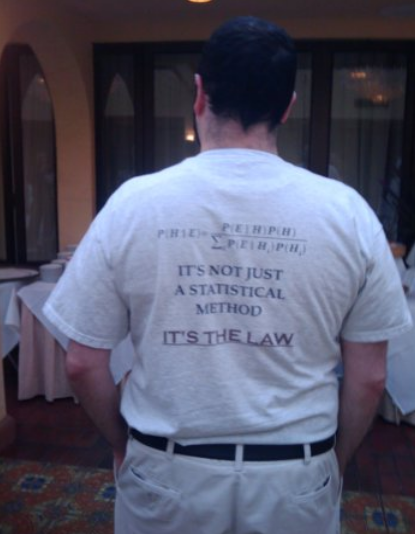
\includegraphics[width=0.4\textwidth]{images/tshirt.png} \\
Credit: lesswrong.com
\end{center}

\end{frame}

\begin{frame}
\begin{center}
\Large
Introduction to MCMC and the Metropolis Algorithm
\end{center}

\end{frame}

\begin{frame}
\frametitle{Philosphy}
\begin{itemize}
\item Markov Chain Monte Carlo (MCMC) algorithms are, strictly speaking, not
Bayesian.\pause
\item However, they are associated with Bayesian statistics because they happen
to be very useful in this area.\pause
\item They allow us to describe posterior distributions in more than one
dimension (more than one unknown parameter) quite easily.
\end{itemize}
\end{frame}

\begin{frame}
\frametitle{More Than One Parameter}
So far we have focused on single-parameter problems until we get used to the
Bayesian approach. But most real problems have more than one unknown parameter.
Imagine making a Bayes Box:
\begin{center}
{\tiny
\begin{tabular}{|c|c|c|c|c|}
\hline
Parameter & Prior & Likelihood & Prior $\times$ Likelihood & Posterior \\
$(\theta_1, \theta_2)$  & $p(\theta_1, \theta_2)$ & $p(x \given \theta_1, \theta_2)$ & $p(\theta_1, \theta_2)p(x\given\theta_1, \theta_2)$ & $p(\theta_1, \theta_2\given x)$ \\
\hline
(0, 0) &  &  & & \\
(0, 0.1) &  &  & & \\
... & ... & ... & ... & ... \\
(0.1, 0) &  &  & & \\
(0.1, 0.1) & & & & \\
... & ... & ... & ... & ... \\
(1, 0.9) & & & & \\
(1, 1) & & & & \\
\hline
Total & 1 & & & 1 \\
\hline
\end{tabular}
} % tiny
\end{center}

\end{frame}

\begin{frame}
\frametitle{More Than One Parameter}
\begin{itemize}
\item Because each hypothesis is about the value of the {\em pair}
$(\theta_1, \theta_2)$, instead of say 100 grid points, we would need
100 $\times$~100. \pause
\item This is quite feasible, but annoying, because you would need 2D arrays
instead of vectors.\pause
\item However, in even higher dimensions (let's say 100) you would need
$10^{100}$ rows (or something like that) in your Bayes Box.
That is not going to happen.
\end{itemize}


\end{frame}


\begin{frame}[fragile]
\frametitle{Grids vs. Samples}
\begin{itemize}
\item You can think of the grid-based approach, which we have used so far,
as assigning {\bf weights} to the $\theta$ values. The posterior probabilities
are the weights, which is why you do calculations like
\mintinline{r}{sum(theta*post)} to get the posterior mean.\pause
\item The purpose of MCMC is to generate {\bf samples} from the posterior
distribution. This is a collection of $\theta$ values that implicitly have
equal weight. To get the posterior mean you would just do \mintinline{r}{mean(theta)}.
This is called {\bf Monte Carlo}.
\end{itemize}


\end{frame}


\begin{frame}[fragile]
\frametitle{Grids vs. Samples}
\centering
\includegraphics[width=0.6\textwidth]{images/grid_vs_samples.pdf}

\end{frame}

\begin{frame}
\frametitle{Using Monte Carlo Samples}
\begin{itemize}
\item If we can generate random numbers from the
posterior, then the histogram will look just like the posterior.\pause
\item If we have enough random numbers, we can use the
sample mean which will be almost the same as the
actual posterior mean.\pause
\item Same with sd or any other summary.
\end{itemize}

\end{frame}

\begin{frame}
\frametitle{Monte Carlo}
\centering
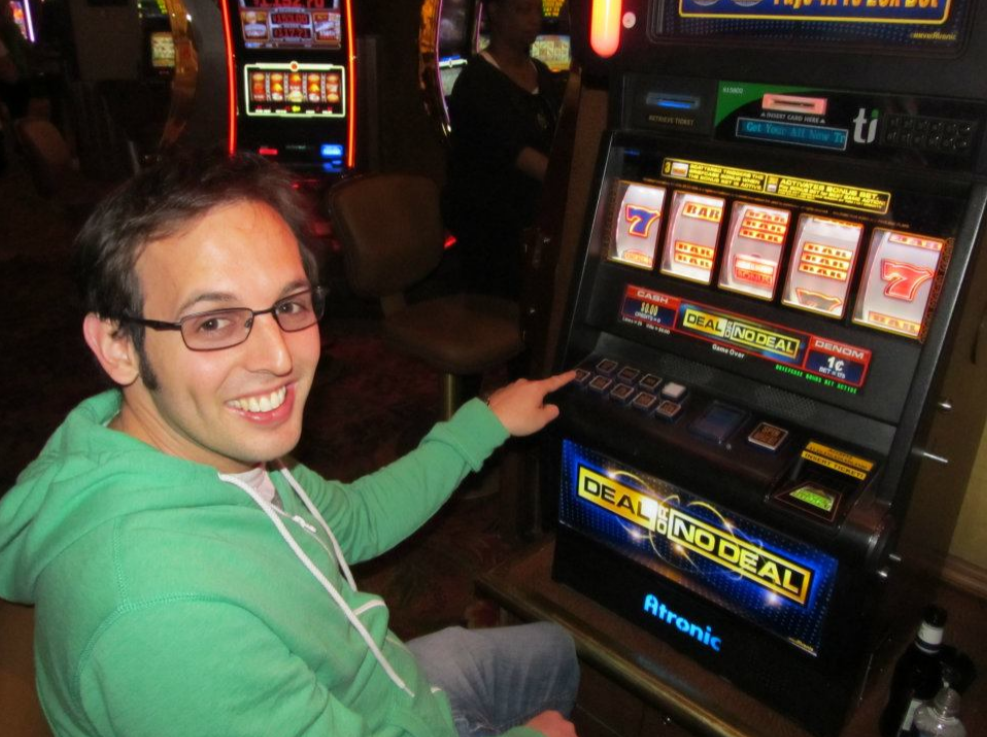
\includegraphics[width=0.6\textwidth]{images/vegas.png}

I was actually in Las Vegas, not Monte Carlo.

\end{frame}

\begin{frame}
\frametitle{Large Sample Size}

\begin{itemize}
\item More samples means the generated $\theta$ values more accurately
reflect the posterior.\pause
\item But the posterior still has the uncertainty built into it, as represented
by the scatter in the generated $\theta$ values.\pause
\item We will assume that we always have a `large enough'
sample from the posterior. It is possible to worry about extra
uncertainty from the Monte Carlo approximation itself, but we will ignore this.
\end{itemize}

\end{frame}



\begin{frame}
\frametitle{Marginalisation}
Marginalisation is the process of going from a higher dimensional probability
distribution to a lower dimensional one. Consider the following table,
with a parameter $\theta_1$ on the $x$-axis and $\theta_2$ on the $y$-axis.
\begin{align}
\begin{array}{c|cccc}
4 & 1/16 & 1/12 & 1/8 & 1/4 \\
3 & 1/16 & 1/12 & 1/8 & 0 \\
2 & 1/16 & 1/12 & 0   & 0 \\
1 & 1/16 & 0    & 0   & 0 \\
\hline
  & 1    & 2    & 3   & 4
\end{array}
\end{align}
\pause
If we only really care about $\theta_1$, we sum the columns
to get the {\bf marginal distribution}.


\end{frame}


\begin{frame}
\frametitle{Marginalisation}
The result of the marginalisation is the following probability distribution
for $\theta_1$ by itself:

\begin{center}
\begin{align}
\left\{\frac{1}{4}, \frac{1}{4}, \frac{1}{4}, \frac{1}{4}\right\}
\end{align}
\end{center}

\end{frame}


\begin{frame}
\frametitle{General Marginalisation}
If there are parameters $\theta_1, ..., \theta_N$ that we care about,
and ``nuisance parameters'' $\phi_1, ..., \phi_M$ that we don't, we can
{\bf integrate out} the nuisance parameters (this is similar to the column
sum we just did).
\pause
\begin{align}
p(\theta_1, ..., \theta_N \given x)
    &= \int p(\theta_1, ..., \theta_N, \phi_1, ..., \phi_M \given x)
            \, d\phi_1 ... d\phi_M.
\end{align}
\pause
One of the benefits of Monte Carlo is that we can avoid doing this integral.
\end{frame}



\begin{frame}
\frametitle{Marginalisation}
\centering
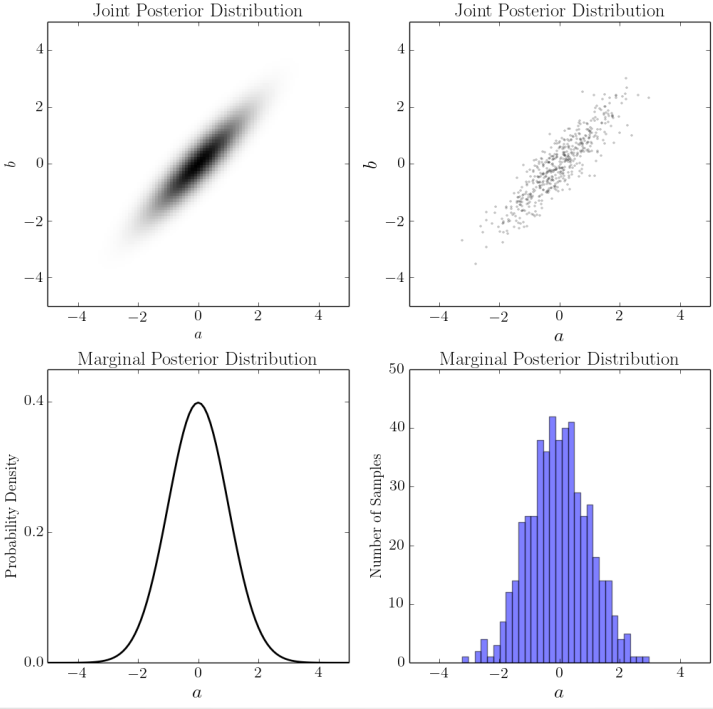
\includegraphics[width=0.6\textwidth]{images/marginalisation.png}

\end{frame}

\begin{frame}
\frametitle{Marginalisation}
Our samples will usually be in a 2D array format (or an R data frame),
where each row is one sample from the joint posterior and each column is
a particular parameter.
To get a marginal distribution we simply look at one column at a time.
This is a lot easier than multiple integration!

\end{frame}


\begin{frame}
\frametitle{Markov Chain}
{\bf Monte Carlo} is about the use of samples to approximate a probability
distribution (for us, almost always the posterior distribution). Markov chains
are used when we actually generate the samples.
\pause

A Markov Chain is sequence of `random variables', where each one
depends on the previous one but not on the ones before that.
A general joint distribution:
\begin{align}
p(x_1, x_2, x_3, x_4) &= p(x_1)p(x_2 \given x_1)p(x_3 \given x_2, x_1)
                    p(x_4 \given x_3, x_2, x_1)
\end{align}
A Markov Chain:
\begin{align}
p(x_1, x_2, x_3, x_4) &= p(x_1)p(x_2 \given x_1)p(x_3 \given x_2)p(x_4 \given x_3).
\end{align}


\end{frame}


\begin{frame}
\frametitle{An Example Markov Chain}
A {\bf random walk} is an example of a Markov Chain.

\begin{itemize}
\item Start at position $x=0$.\pause
\item Flip a coin.\pause
\item Heads? Add 1. Tails? Subtract 1.\pause
\end{itemize}

You will get a sequence like this:
0, -1, 0, 1, 2, 3, 2, 1, 2, 3, 4, 3, 4, ...
\pause

The thing that is a Markov Chain is the probability distribution for the
sequence, not a given sequence itself.

\end{frame}

\begin{frame}
\frametitle{Markov Chains: Stationary Distribution}
Markov Chains often have a {\bf stationary distribution}.

\begin{itemize}
\item If you start with an initial point specified probabilistically
with the stationary distribution, then the distribution for `where I go next'
is also the stationary distribution.\pause
\item It is the probability distribution representing where the
algorithm will be after a long time.\pause
\item With high probability, it is also the
frequency distribution of results you get
after running the chain for a long time.
\end{itemize}


\end{frame}

\begin{frame}
\frametitle{MCMC Target Distributions}
The key idea of MCMC is to engineer a Markov Chain whose stationary distribution
is the {\bf target distribution} that you are interested in --- for us, this
will mostly be a posterior distribution. There are a few different ways to do
this. We will study the {\bf Metropolis algorithm}.

\end{frame}




\begin{frame}
\frametitle{The Metropolis Algorithm}
The {\bf Metropolis Algorithm} (sometimes {\bf Metropolis-Hastings})
is one of the most famous and general
MCMC methods available, invented in the 1950s. The output looks like a Metropolis:
\begin{center}
\includegraphics[width=0.6\textwidth]{images/metropolis.pdf}
\end{center}

\end{frame}

\begin{frame}
\frametitle{The Metropolis Algorithm}
That is just a coincidence.
It is actually named after Nicholas Metropolis.

\begin{center}
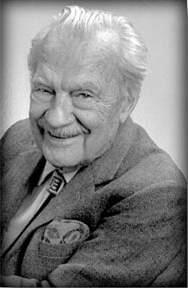
\includegraphics[width=0.2\textwidth]{images/nicholas_metropolis.png}

(Public domain image)
\end{center}

\end{frame}


\begin{frame}
\frametitle{The Metropolis Algorithm}
\begin{itemize}
\item We want to sample the posterior distribution for a Bayesian inference problem. \pause
\item Start with something we {\em can} do, called the {\bf proposal distribution.}\pause
\item Use {\bf acceptance and rejection} to modify the distribution into the
one we want.\pause
\item To implement Metropolis, we assume that a function exists which returns
the prior times likelihood value for whatever value of parameters $\theta$
we pass in.
\end{itemize}

\end{frame}

\begin{frame}
\frametitle{An Example Proposal Distribution}

\begin{itemize}
\item As a simple example, suppose $\theta \in \{1, 2, 3, 4, 5\}$, and our proposal
distribution is a wrapped random walk (so if you are at 5 and you try to add
one, it wraps back to 1).\pause
\item If we let this happen for a long time, we will end up with a uniform
(frequency) distribution of $\theta$ values, because that is the
{\bf stationary distribution} of this Markov Chain.\pause
\item Putting in acceptance and rejection modifies the stationary distribution
of the Markov Chain so that it becomes the target distribution of interest
(the posterior).
\end{itemize}

\end{frame}


\begin{frame}
\frametitle{Acceptance and Rejection}
\centering
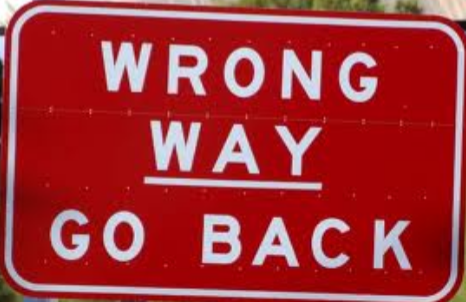
\includegraphics[width=0.7\textwidth]{images/wrong_way.png}

\end{frame}

\begin{frame}
\frametitle{Acceptance and Rejection}
Call the prior times likelihood function $h(\theta)$.
If we try to move from $\theta$ to $\theta'$ because the proposal distribution
resulted in $\theta'$, we only accept it with the following probability:
\begin{align}
P(\textnormal{accept}) &= \min\left(1, \frac{h(\theta')}{h(\theta)}\right)
\end{align}
\pause

That is, uphill moves are accepted. Downhill moves are accepted with a probability
based on the ratio of prior $\times$ likelihood values.

\end{frame}

\begin{frame}
\frametitle{Example Distribution to Sample}
Example target/posterior distribution. Here are the prior times likelihood
values:
\begin{align}
h &= \{ 0.1, 0.2, 0.3, 0.3, 0.1 \}
\end{align}

\end{frame}


\begin{frame}
\frametitle{Metropolis Process}
\begin{center}
\begin{align}
h &= \{ 0.1, 0.2, 0.3, 0.3, 0.1 \}
\end{align}
{\tiny
\begin{tabular}{|c|c|c|c|c|}
\hline
Iteration & State & Proposal & Acceptance Probability & Accepted? \\
\hline 
1         & 1     & 5        & 1                      & Yes \\
2         & 1     & 2        & 1                      & Yes \\
3         & 2     & 1        & 1/2                    & No \\
4         & 2     & 3        & 1                      & Yes \\
5         & 3     & 2        & 2/3                    & Yes \\
6         & 2     & 1        & 1                      & Yes \\
7         & 1     & 5        & 1                      & Yes \\
8         & 5     & 4        & 1                      & Yes \\
9         & 4     & 5        & 1/3                    & No \\
10        & 4     & ... & ... & ... \\
... & ... & ... & ... & ...  \\
\hline
\end{tabular}
} % tiny
\end{center}
\pause

Note: The sampler spends more time in high probability states, precisely
because moving away from these states is often rejected.
\end{frame}


\begin{frame}[fragile]
\frametitle{Metropolis Code}

I will now implement a simple toy version of the Metropolis algorithm in R
to sample from a standard normal distribution. The $h$ function looks like this:

\begin{minted}{r}
prior_times_likelihood = function(theta)
{
    return(exp(-0.5*theta^2))
}
\end{minted}
\pause

In more serious code such as the ``industrial strength'' Metropolis code on
Canvas, it is usually the {\em log} of $h$ that is used.
\end{frame}



\begin{frame}[fragile]
\frametitle{Metropolis Code: Main Loop}

\small
\begin{minted}{r}
theta = 0 # Some starting point
h1 = prior_times_likelihood(theta)
for(i in 1:100000)
{
    proposal = theta + rnorm(1)
    h2 = prior_times_likelihood(proposal)
    if(runif(1) <= h2/h1)
    {
        theta = proposal  # Accept the proposal
        h1 = h2
    } # Rejection requires no code
}
\end{minted}

\end{frame}

\begin{frame}[fragile]
\frametitle{Metropolis Code: Saving Results (in RAM)}
\begin{minted}{r}
steps = 100000
keep = numeric(steps)
for(i in 1:steps)
{
    # ...
    keep[i] = theta
}
\end{minted}
\end{frame}


\begin{frame}[fragile]
\frametitle{Trace Plots}
A {\bf trace plot} is simply a plot of a parameter over time as the MCMC
proceeds. They are easy to produce:
\begin{minted}{r}
plot(keep, type="l", xlab="Iteration", ylab="theta")
\end{minted}

\end{frame}

\begin{frame}[fragile]
\frametitle{An Example Trace Plot}
This is what a trace plot looks like when things are working well.

\begin{center}
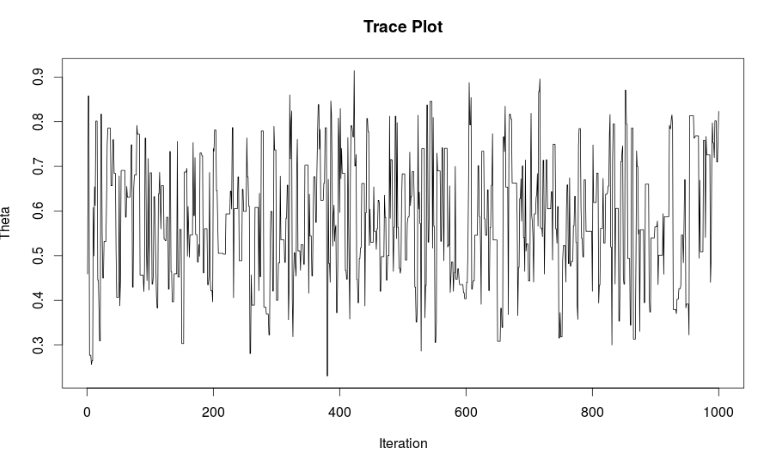
\includegraphics[width=0.8\textwidth]{images/trace_plot.png}
\end{center}

Some people call it a ``fuzzy caterpillar''. It looks a bit more like that
if you have a longer run and zoom out.

\end{frame}



\begin{frame}[fragile]
\frametitle{Autocorrelation Plots}
The {\bf autocorrelation function} can tell us about how well the algorithm
is moving around. We want the autocorrelation to drop to zero quickly, ideally.

\begin{minted}{r}
acf(keep, lag.max=100)
\end{minted}

\end{frame}




\begin{frame}[fragile]
\frametitle{Metropolis Code: Acceptance Rate}
The acceptance rate can be monitored for diagnostic purposes.
\small
\begin{minted}{r}
# ...
accepted = 0
for(i in 1:steps)
{
    # ...
    if(runif(1) <= h2/h1)
    {
        accepted = accepted + 1
    } # Rejection requires no code
}
acceptance_rate = accepted / steps
\end{minted}

\end{frame}




\begin{frame}
\frametitle{Running MCMC}
Let's now run MCMC to see how it performs. In particular, we will look at
the following phenomena:
\begin{itemize}
\item `Burn-in', which occurs when the starting point is not in a typical region
of the target/posterior distribution.\pause
\item What happens when the proposal distribution is (i) too narrow,
(ii) just right, or (iii) too wide.
\end{itemize}
\pause
What happens to the trace plots, the autocorrelation plots, and the acceptance
rate?

\end{frame}



\begin{frame}
\frametitle{MCMC Phenomena}
\begin{itemize}
\item If the starting point is bad, there might be a burn-in period (sometimes
quite long). \pause
\item If the proposal is too wide, too many proposals are rejected, so the
algorithm stays stuck for long periods of time.\pause
\item If it is too narrow, too many proposals are accepted (remember it is
the {\em pattern} of acceptance and rejection that shapes the distribution
into what we want), and they do not move very far.
\end{itemize}

\end{frame}

\begin{frame}
\frametitle{MCMC Tuning}

\centering

\includegraphics[width=0.5\textwidth]{images/goldilocks.png}

Image credit: Global Legal Post

\end{frame}



\begin{frame}[fragile]
\frametitle{Tuning the Proposal Distribution}
Often, people will perform some preliminary experiments to figure out how
wide the proposal distribution should be for Metropolis to perform efficiently.
In the simple Metropolis code we have, this would mean tweaking the
coefficient in front of \mintinline{r}{rnorm()}. For example:

\begin{minted}{r}
proposal = theta + 10*rnorm(1)
\end{minted}

\end{frame}



\begin{frame}[fragile]
\frametitle{Randomising the Proposal Distribution}
An alternative to using preliminary runs is to use a heavy-tailed proposal
distribution. One easy way to achieve this is to randomly choose the step
size each iteration, so it is sometimes small and sometimes big.
Here's an example using a lognormal distribution:

\begin{minted}{r}
sigma = exp(3*rnorm(1))
proposal = theta + sigma*rnorm(1)
\end{minted}

\pause

This still assumes that the optimal step size is within a couple of orders
of magnitude of 1. The industrial strength implementation on Canvas does this.

\end{frame}


\begin{frame}[fragile]
\frametitle{Proposal Distribution for Many Parameters}
The whole point of MCMC was to extend our ability to solve problems to the
situation with many unknown parameters. So how does the proposal work in this
case? You can move all parameters at once, or pick one randomly each time.

{\small
\begin{minted}{r}
# Choose which parameter to change
k = sample(1:length(params), 1)

# Change it
step_size = step_sizes[k]*exp(scale_step_sizes[k]*rt(1, df=2))
params[k] = params[k] + step_size*rnorm(1)
\end{minted}
} % small

\end{frame}





\begin{frame}[fragile]
\frametitle{Metropolis Code: Thinning}
\begin{minted}{r}
steps = 100000
skip = 100
keep = numeric(steps %/% skip)
for(i in 1:steps)
{
    # ...
    if(i %% skip == 0)
        keep[i %/% skip] = theta
}
\end{minted}
\end{frame}


\begin{frame}[fragile]
\frametitle{Metropolis Code: Thinning}
\begin{itemize}
\item Thinning is used to prevent the output from getting too big.
Because the MCMC samples are correlated, we sometimes need a large number
of steps, but we do not need to save every step. \pause
\item If you use \mintinline{r}{acf()} after thinning, remember that each unit
of lag will really be \mintinline{r}{skip} iterations of MCMC.
\end{itemize}
\end{frame}



\begin{frame}[fragile]
\frametitle{Data Analysis}
Let's solve an actual data analysis problem using the industrial strength
MCMC code. We'll do the election poll problem, which is still only 1D --- you
will do your first 2D analysis in labs. The \mintinline{r}{log_prob} function
needs to look like this:
{\footnotesize
\begin{minted}{r}
log_prob = function(params)
{
    # Return -Inf if parameter is out of bounds.
    if(params["theta"] <= 0 || params["theta"] >= 1)
        return(-Inf)
    log_prior = 0
    log_likelihood = 6*log(params["theta"]) + 4*log(1 - params["theta"])
    return(log_prior + log_likelihood)
}
\end{minted}
} %footnotesize

\end{frame}


\begin{frame}[fragile]
\frametitle{Posterior Summaries and Plots}

\begin{minted}{r}
results = read.csv("metropolis-output.csv")
plot(results$theta, type="l")
hist(results$theta, breaks=100)
mean(results$theta)
sd(results$theta)
\end{minted}

\end{frame}



\end{document}

